%iffalse
\let\negmedspace\undefined
\let\negthickspace\undefined
\documentclass[journal,12pt,onecolumn]{IEEEtran}
\usepackage{cite}
\usepackage{amsmath,amssymb,amsfonts,amsthm}
\usepackage{algorithmic}
\usepackage{multicol}
\usepackage{circuitikz}
\usepackage{tikz}
\usepackage{graphicx}
\usepackage{textcomp}
\usepackage{xcolor}
\usepackage{txfonts}
\usepackage{listings}
\usepackage{enumitem}
\usepackage{mathtools}
\usepackage{gensymb}
\usepackage{comment}
\usepackage[breaklinks=true]{hyperref}
\usepackage{tkz-euclide} 
\usepackage{listings}
\usepackage{gvv}                                        
%\def\inputGnumericTable{}                                 
\usepackage[latin1]{inputenc}                                
\usepackage{color}                                            
\usepackage{array}                                            
\usepackage{longtable}                                       
\usepackage{calc}                                             
\usepackage{multirow}                                         
\usepackage{hhline}                                           
\usepackage{ifthen}                                           
\usepackage{lscape}
\usepackage{tabularx}
\usepackage{array}
\usepackage{float}
\newtheorem{theorem}{Theorem}[section]
\newtheorem{problem}{Problem}
\newtheorem{proposition}{Proposition}[section]
\newtheorem{lemma}{Lemma}[section]
\newtheorem{corollary}[theorem]{Corollary}
\newtheorem{example}{Example}[section]
\newtheorem{definition}[problem]{Definition}
\newcommand{\BEQA}{\begin{eqnarray}}
\newcommand{\EEQA}{\end{eqnarray}}
\newcommand{\define}{\stackrel{\triangle}{=}}
\theoremstyle{remark}
\newtheorem{rem}{Remark}

% Marks the beginning of the document
\begin{document}
\bibliographystyle{IEEEtran}
\vspace{3cm}

\title{\textbf{EE-2007 52-68}}
\author{AI24BTECH11012- Pushkar Gudla}
\maketitle
\bigskip

\renewcommand{\thefigure}{\theenumi}
\renewcommand{\thetable}{\theenumi}
\setlength{\columnsep}{2.5em}

\begin{enumerate}
    \item The integral$
    \frac{1}{2\pi} \int_{0}^{2\pi} \sin(t - \tau)\cos \tau , d\tau$
    equals:
    
    \begin{enumerate}
        \item $\sin t \cos t$
        \item $0$
        \item $\frac{1}{2} \cos t$
        \item $\frac{1}{2} \sin t$
    \end{enumerate}
    
    \item $X(z) = 1 - 3z^{-1}, \, Y(z) = 1 + 2z^{-2}$ are Z-transforms of two signals $x[n], y[n]$ respectively. A linear time invariant system has the impulse response $h[n]$ defined by these two signals as:
 \[
    h[n] = x[n - 1] * y[n]
 \]
    where $*$ denotes discrete time convolution. Then the output of the system for the input $\delta[n - 1]$ is:
    
    \begin{enumerate}
        \item Has Z-transform $z^{-1} X(z)Y(z)$
        \item Equals $\delta[n - 2] - 3\delta[n - 3] + 2\delta[n - 4] - 6\delta[n - 5]$
        \item Has Z-transform $1 - 3z^{-1} + 2z^{-2} - 6z^{-3}$
        \item Does not satisfy any of the above three
    \end{enumerate}
    
    \item A loaded dice has the following probability distribution of occurrences:
    
    \[
    \begin{array}{|c|c|c|c|c|c|c|}
    \hline
    \text{Dice value} & 1 & 2 & 3 & 4 & 5 & 6 \\
    \hline
    \text{Probability} & \frac{1}{4} & \frac{1}{8} & \frac{1}{8} & \frac{1}{8} & \frac{1}{8} & \frac{1}{4} \\
    \hline
    \end{array}
    \]
    
    If three identical dice as the above are thrown, the probability of occurrence of values 1, 5, and 6 on the three dice is:
    
    \begin{enumerate}
        \item Same as that of occurrence of $3, 4, 5$
        \item Same as that of occurrence of $1, 2, 5$
        \item $\frac{1}{128}$
        \item $\frac{5}{8}$
    \end{enumerate}
        \item Let $x$ and $y$ be two vectors in a 3-dimensional space and $< x, y >$ denote their dot product. Then the determinant

    \[
    \det \begin{bmatrix}
    < x, x > & < x, y > \\
    < y, x > & < y, y >
    \end{bmatrix}
    \]

    \begin{enumerate}
        \item is zero when $x$ and $y$ are linearly independent
        \item is positive when $x$ and $y$ are linearly independent
        \item is non-zero for all non-zero $x$ and $y$
        \item is zero only when either $x$ or $y$ is zero
    \end{enumerate}

    \item The linear operation $L(x)$ is defined by the cross product $L(x) = \mathbf{b} \times x$, where $\mathbf{b} = [0 , 1 , 0]^T$ and $x = [x_1 , x_2 , x_3]^T$ are three-dimensional vectors. The $3 \times 3$ matrix $\mathbf{M}$ of this operation satisfies:

    \[
    L(x) = \mathbf{M} 
    \begin{bmatrix}
    x_1 \\
    x_2 \\
    x_3
    \end{bmatrix}
    \]

    Then the eigenvalues of $\mathbf{M}$ are:

    \begin{enumerate}
        \item $0, +1, -1$
        \item $1, -1, 1$
        \item $i, -i, 1$
        \item $i, -i, 0$
    \end{enumerate}
\item In the figure, transformer $T_1$ has two secondaries all three windings having the same number of turns and with polarities as indicated. One secondary is shorted by a $10 \ohm$ resistor R, and the other by a $15 \mu F$ capacitor. The switch SW is opened $\brak{t=0}$ when the capacitor is charged to $5V$ with the left plate as positive. At $t=0+$ the voltage $V_p$ and current $I_R$ are
\begin{figure}[!ht]
\centering
\resizebox{0.5\textwidth}{!}{%
\begin{circuitikz}
\tikzstyle{every node}=[font=\LARGE]
\draw (1.25,16) to[battery1] (1.25,14.5);
\draw (1.25,16) to[opening switch] (3.25,16);
\node [font=\small] at (0.25,15.25) {25 V};
\draw (3.25,16) to[R] (3.75,16);
\draw (4,16) to[L ] (4,14.5);
\draw (1.25,14.5) to[short] (4,14.5);
\draw [short] (4.5,16.25) -- (4.5,14.5);
\draw [short] (4.75,16.25) -- (4.75,14.5);
\node [font=\small] at (2,16.75) {SW};
\node [font=\small] at (4.5,16.75) {$T_1$};
\draw (5.25,16.25) to[L ] (5.25,15.75);
\draw (5.25,16.5) to[R] (6.5,16.5);
\draw (6.5,16.5) to[short] (6.5,15.5);
\draw (5.25,15.5) to[short] (6.5,15.5);
\node [font=\small] at (6.5,16.75) {R};
\draw [->, >=Stealth] (5.25,17.25) -- (6.75,17.25);
\node [font=\small] at (6,17.75) {IR};
\draw (5.25,15) to[L ] (5.25,14.5);
\draw (5.25,15.25) to[C] (6.5,15.25);
\draw (6.5,15.25) to[short] (6.5,14.25);
\draw (5.25,14.25) to[short] (6.5,14.25);
\node [font=\small] at (6.5,15.25) {C};
\end{circuitikz}
}%

\label{fig:my_label}
\end{figure}

\begin{enumerate}
\item $-25 V, 0.0 A$
\item very large voltage, very large current
\item $5.0 V, 0.5 A$
\item $-5.0 V, -5.0 A$
\end{enumerate}

\item IC $555$ in the adjacent figure is configured as an astable
multivibrator. it is enabled to oscillate at $t=0$ by applying a high input to pin 4. The pin description is: 1 and 8-supply; 2-trigger; 4-reset; 6-threshold; 7-discharge. The waveform appearing across the capacitor starting from $t=0$, as observed on a storage CRO is:
\begin{figure}[!ht]
\resizebox{0.4\textwidth}{!}{%
\begin{circuitikz}
\tikzstyle{every node}=[font=\large]
\draw [short] (4.25,16.5) -- (4.25,14);
\draw [short] (4.25,16.5) -- (6.5,16.5);
\draw [short] (6.5,16.5) -- (6.5,14);
\draw [short] (4.25,14) -- (6.5,14);
\node [font=\small] at (5.5,15.25) {IC 555};
\draw [short] (5.25,17.25) -- (5.25,16.5);
\draw [short] (3.5,17.25) -- (5.25,17.25);
\draw [->, >=Stealth] (3.25,16.5) -- (3.25,18);
\draw [short] (3.25,17.25) -- (3.5,17.25);
\draw  (3,16.5) rectangle (3.5,15.75);
\draw [short] (3.25,15.75) -- (3.25,14.5);
\draw [short] (2.75,15.25) -- (4.25,15.25);
\draw  (3,14.5) rectangle (3.25,13.5);
\draw [short] (2.75,15.25) -- (2.5,15.25);
\draw [short] (2.5,15.25) -- (2.5,14.75);
\draw (2.5,14.75) to[D] (2.5,13.75);
\draw [short] (2.5,13.75) -- (4.25,14.25);
\draw [short] (4.75,14) -- (4.75,12.75);
\draw [short] (4.75,12.75) -- (2.75,12.75);
\draw (3,13.5) to[C] (3,13);
\draw (3,13) to (3,12.75) node[ground]{};
\node [font=\normalsize] at (2.5,16.25) {10 K};
\node [font=\normalsize] at (4,13.5) {10 K};
\end{circuitikz}
}%

\label{fig:my_label}
\end{figure}

\begin{enumerate}
\item 
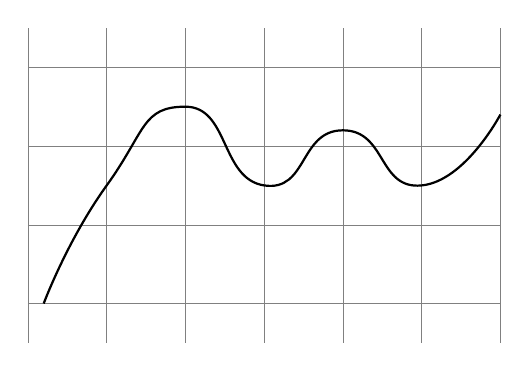
\begin{tikzpicture}
    % Grid
    \draw[very thin, gray] (-2, -1.5) grid (4, 2.5);
    
    % Plot the curve (example curve for approximation)
    \draw[thick] plot[smooth, tension=1] coordinates {(-1.8,-1) (-1, 0.5) (0, 1.5) (1, 0.5) (2, 1.2) (3, 0.5) (4, 1.4)};
    
\end{tikzpicture}
\item 
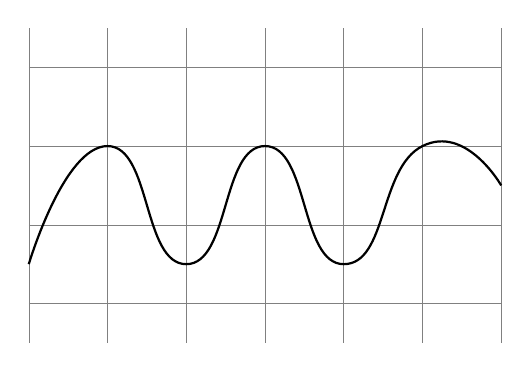
\begin{tikzpicture}
    % Grid
    \draw[very thin, gray] (-2, -1.5) grid (4, 2.5);
    
    % Plot the wave-like curve
    \draw[thick] plot[smooth, tension=1] coordinates {(-2, -0.5) (-1, 1) (0, -0.5) (1, 1) (2, -0.5) (3, 1) (4, 0.5)};
    
\end{tikzpicture}
\item 
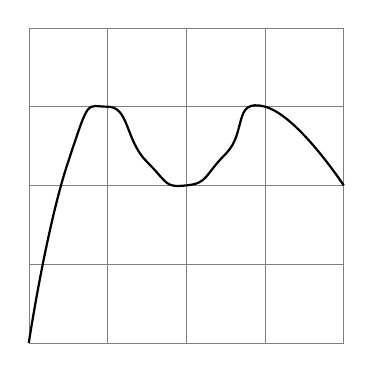
\begin{tikzpicture}
    % Grid
    \draw[very thin, gray] (-2, -2) grid (2, 2);

    % Plot the wave-like curve with a sharper point at (-1, 1)
    \draw[thick] plot[smooth, tension=1] coordinates {
        (-2, -2)
        (-1.5, 0.3)  % Added control point
        (-1, 1)
        (-0.5, 0.3)
        (0,0)
        (0.5,0.4)
        (1, 1)
        (2, 0)
    };
\end{tikzpicture}
\item 
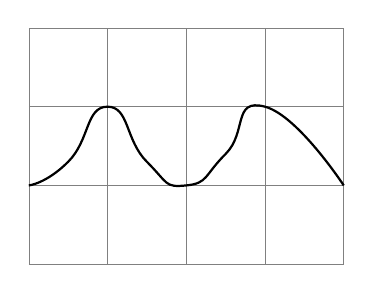
\begin{tikzpicture}
    % Grid
    \draw[very thin, gray] (-2, -1) grid (2, 2);

    % Plot the wave-like curve with a sharper point at (-1, 1)
    \draw[thick] plot[smooth, tension=1] coordinates {
        (-2, 0)
        (-1.5, 0.3)  % Added control point
        (-1, 1)
        (-0.5, 0.3)
        (0,0)
        (0.5,0.4)
        (1, 1)
        (2, 0)
    };
\end{tikzpicture}
\end{enumerate}

\item In the circuit figure the diode connects the ac source to a pure inductance L. The diode conducts for
\begin{figure}[!ht]
\centering
\resizebox{0.2\textwidth}{!}{%
\begin{circuitikz}
\tikzstyle{every node}=[font=\normalsize]
\draw (2,16.5) to[D] (4.25,16.5);
\draw (2,16.5) to[short] (4,16.5);
\draw (2,16.5) to[short] (2,16);
\draw  (2,15.75) circle (0.25cm);
\node [font=\LARGE] at (2,15.75) {~};
\node [font=\normalsize] at (1.5,15.75) {AC};
\draw (2,15.5) to[short] (2,14.75);
\draw (2,14.75) to[short] (4.25,14.75);
\draw (4.25,16.5) to[L ] (4.25,14.75);
\end{circuitikz}
}%

\label{fig:my_label}
\end{figure}

\begin{enumerate}
\item $90 \degree$
\item $180 \degree$
\item $270 \degree$
\item $360 \degree$
\end{enumerate}

\item The circuit in the figure is a current commutated dc-dc chopper where, $Th_M$ is the main SCR and $Th_{AUX}$ is the auxiliary SCR. The load current is constant at $10$ A. $Th_M$ is turned OFF between

\begin{figure}[H]
    \centering
    \resizebox{0.3\textwidth}{!}{%
        \begin{circuitikz}
            \tikzstyle{every node}=[font=\small]
            
            % Battery
            \draw (1.25,16.75) to[battery1] (1.25,14.25);
            
            % Diodes and SCRs
            \draw (1.25,16.75) to[D] (6.25,16.75); % Main diode
            \draw (2.5,16.75) to[D] (2.5,15.5); % Auxiliary diode
            \draw (2.5,15.5) to[D] (5,15.5);
            \draw (5,16.75) to[short] (5,14.5);
            
            % Capacitor and Inductor
            \draw (2.5,15.5) to[short] (2.5,14.5);
            \draw (2.5,14.5) to[C, l=10$\mu$F] (3.25,14.5);
            \draw (3.25,14.5) to[L, l=25.28$\mu$H] (5,14.5);
            
            % Load resistor
            \draw (6,13.25) to[D] (6,16.75); % Lower diode
            \draw (6,13.25) to[short] (1.25,13.25);
            \draw (1.25,14.25) to[short] (1.25,13.25);
            \draw (6.25,16.75) to[short] (7,16.75);
            \draw (6,13.25) to[short] (7,13.25);
            \draw (7,16.75) to[european resistor] (7,13.25); % Removed label "l=R"
            
            % Labels
            \node at (0.75,15) {230 V};
            \node at (4,17.25) {$Th_M$};
            \node at (3.75,16) {$Th_{Aux}$};
            \node at (7.5,15.5) {L};
            \node at (7.5,15.25) {O};
            \node at (7.5,15) {A};
            \node at (7.5,14.75) {D};
        \end{circuitikz}
    }
    \label{fig:chopper-circuit}
\end{figure}

    \begin{enumerate}
        \item $0 \mu s<t\leq 25 \mu s$
        \item $25 \mu s<t\leq 50 \mu s$
        \item $50 \mu s<t\leq 75 \mu s$
        \item $75 \mu s<t\leq 100 \mu s$
    \end{enumerate}


\item In the circuit shown in figure switch $SW_1$ is initially CLOSED and $SW_2$ is OPEN. The inductor L carries a current of 10 A and the capacitor is charged to 10 V with polarities as indicated. $SW_2$ is initially CLOSED at $t=0-$ and $SW_1$ is OPENED at $t=0$. The current through C and the voltage across L at $t=0+$ is
\begin{figure}[!ht]
\centering
\resizebox{0.3\textwidth}{!}{%
\begin{circuitikz}
\tikzstyle{every node}=[font=\normalsize]
\draw (1.25,16) to[R] (1.25,14);
\draw (1.25,16) to[short] (2,16);
\draw (1.25,14) to[short] (2,14);
\draw (1.75,16) to[normal open switch] (1.75,14);
\draw (2,16) to[normal open switch] (3.25,16);
\draw (3.25,16) to[R] (4.75,16);
\draw (4.75,16) to[C] (4.75,14);
\draw (2,14) to[short] (4.75,14);
\draw (2.25,16) to[L ] (2.25,14);
\draw [->, >=Stealth] (2.75,14.5) -- (2.75,15.5);
\node [font=\small] at (2.5,14.25) {L};
\node [font=\small] at (3.25,15) {10 emps};
\node [font=\small] at (0.75,15.5) {$R_1 10 \ohm$};
\node [font=\small] at (1.55,14.5) {$SW_1$};
\node [font=\small] at (2.5,16.25) {$SW_2$};
\node [font=\small] at (4,16.75) {$R_2 10 \ohm$};
\node [font=\small] at (4.25,14.75) {C};
\node [font=\small] at (5.5,14.75) {10 V};
\end{circuitikz}
}%

\label{fig:my_label}
\end{figure}

\begin{enumerate}
\item $55 A, 4.5 V$
\item $5.5 A, 45 V$
\item $45 A, 5.5 V$
\item $4.5 A, 55V$
\end{enumerate}

\item The R-L-C series circuit shown is supplied from a variable frequency voltage source. The admittance-locus of the R-L-C network at terminals AB for increasing frequency $w$ is
\begin{figure}[!ht]
\centering
\resizebox{0.3\textwidth}{!}{%
\begin{circuitikz}
\tikzstyle{every node}=[font=\small]
\draw (1,18.75) to[sinusoidal voltage source, sources/symbol/rotate=auto] (1,15.5);
\draw (1,18.75) to[R] (5.25,18.75);
\draw (1,15.5) to[C] (5.25,15.5);
\draw (5.25,18.75) to[L ] (5.25,15.5);
\node [font=\small] at (3,18.25) {$R$};
\node [font=\small] at (2,17.25) {$$w$$};
\node [font=\small] at (3,14.75) {$C$};
\node [font=\small] at (6,17.25) {$L$};
\end{circuitikz}
}%

\label{fig:my_label}
\end{figure}

\begin{enumerate}

\item \begin{circuitikz}
\tikzstyle{every node}=[font=\normalsize]
\draw [short] (2,17) -- (2,13.5);
\draw [short] (0.75,14.75) -- (4.75,14.75);
\draw  (2.75,14.75) ellipse (0.75cm and 1cm);
\draw [->, >=Stealth] (2.75,13.75) -- (3,13.75);
\node [font=\normalsize] at (3.5,13.75) {w};
\draw [->, >=Stealth] (3.75,14.25) -- (4.75,14.25);
\node [font=\normalsize] at (4.5,13.75) {Re};
\draw [->, >=Stealth] (1.75,16) -- (1.75,17);
\node [font=\normalsize] at (1,16.25) {Im};
\end{circuitikz}



\item 
\begin{circuitikz}
\tikzstyle{every node}=[font=\normalsize]
\draw [short] (2,17) -- (2,13.5);
\draw [short] (0.75,14.75) -- (4.75,14.75);
\draw  (2.75,14.75) ellipse (0.75cm and 1cm);
\node [font=\normalsize] at (3.5,13.75) {w};
\draw [->, >=Stealth] (3.75,14.25) -- (4.75,14.25);
\node [font=\normalsize] at (4.5,13.75) {Re};
\draw [->, >=Stealth] (1.75,16) -- (1.75,17);
\node [font=\normalsize] at (1,16.25) {Im};
\draw [->, >=Stealth] (2.75,13.75) -- (2.5,13.75);
\end{circuitikz}



\item 
\begin{circuitikz}
\tikzstyle{every node}=[font=\normalsize]
\draw [short] (2,17) -- (2,13.5);
\draw [short] (0.75,14.75) -- (4.75,14.75);
\draw  (2,15.75) ellipse (0.75cm and 1cm);
\node [font=\normalsize] at (3.25,16) {w};
\draw [->, >=Stealth] (3.75,14.25) -- (4.75,14.25);
\node [font=\normalsize] at (4.5,13.75) {Re};
\draw [->, >=Stealth] (1.75,16) -- (1.75,17);
\node [font=\normalsize] at (1,16.25) {Im};
\draw [->, >=Stealth] (2.75,15.75) -- (2.75,16);
\end{circuitikz}



\item 
\begin{circuitikz}
\tikzstyle{every node}=[font=\normalsize]
\draw [short] (2,17) -- (2,13.5);
\draw [short] (0.75,14.75) -- (4.75,14.75);
\draw  (2,15.75) ellipse (0.75cm and 1cm);
\node [font=\normalsize] at (1,15.25) {w};
\draw [->, >=Stealth] (3.75,14.25) -- (4.75,14.25);
\node [font=\normalsize] at (4.5,13.75) {Re};
\draw [->, >=Stealth] (1.75,16) -- (1.75,17);
\node [font=\normalsize] at (1,16.25) {Im};
\draw [->, >=Stealth] (2,11) -- (2,11.25);
\draw [->, >=Stealth] (1.25,15.5) -- (1.25,15.75);
\end{circuitikz}

\end{enumerate} 
\item In the figure given below all phasors are with reference to the potential at point "O". The locus of voltage phasor $\mathbf{V_{YX}}$ as R is varied from zero to infinity is shown by

\begin{circuitikz}
\tikzstyle{every node}=[font=\small]
\draw (2,16.75) to[short] (4.75,16.75);
\draw (4.75,16.75) to[short] (4.75,16.25);
\draw (2,16.75) to[sinusoidal voltage source, sources/symbol/rotate=auto] (2,15.25);
\draw (2,15.25) to[sinusoidal voltage source, sources/symbol/rotate=auto] (2,14);
\draw (2,15.25) to[short, -o] (3,15.25) ;
\draw  (4.5,16.25) rectangle (5,15.5);
\draw [->, >=Stealth] (4.25,15.75) -- (5.5,16);
\node [font=\small] at (4.75,16) {R};
\draw (4.75,15.5) to[short] (4.75,15);
\draw (4.75,15) to[short, -o] (3.75,15) ;
\draw (4.75,15) to[C] (4.75,14);
\draw (2,14) to[short] (4.75,14);
\node [font=\small] at (5.25,14.25) {C};
\node [font=\small] at (3.5,13.75) {O};
\node [font=\small] at (1,14.75) {$V< 0\degree$};
\draw [->, >=Stealth] (1.5,14.25) -- (1.5,15);
\draw [->, >=Stealth] (1.5,15.75) -- (1.5,16.5);
\draw [->, >=Stealth] (3,15.5) -- (4,15.5);
\node [font=\small] at (3.5,15.75) {$V_{xy}$};
\node [font=\small] at (3,14.75) {X};
\node [font=\small] at (4,14.75) {Y};
\node [font=\small] at (1,16.25) {$V<0\degree$ } ;
\end{circuitikz}

\begin{enumerate}

\item 
\begin{circuitikz}
\tikzstyle{every node}=[font=\small]
\draw [dashed] (1.12,16.25) arc[start angle=180, end angle=360, radius=1.75cm];
\draw [->, >=Stealth] (1.25,16.25) -- (4.75,16.25);
\draw [->, >=Stealth] (2.75,16.25) -- (1.75,15);
\node [font=\small] at (1,16.25) {O};
\node [font=\small] at (5,16.25) {2V};
\node [font=\small] at (2.5,15.75) {$V_{YX}$};
\end{circuitikz}


\item
\begin{circuitikz}
\tikzstyle{every node}=[font=\small]
\draw [dashed] (4.62,16.25) arc[start angle=0, end angle=180, radius=1.75cm];
\draw [->, >=Stealth] (1.25,16.25) -- (4.75,16.25);
\node [font=\small] at (1,16.25) {Ot};
\node [font=\small] at (5,16.25) {2V};
\node [font=\small] at (3,17) {$V_{YX}$};
\draw [->, >=Stealth] (3,16.25) -- (2,17.75);
\end{circuitikz}


\item 
\begin{circuitikz}
\tikzstyle{every node}=[font=\small]
\draw [dashed] (1.12,16.25) arc[start angle=180, end angle=360, radius=1.75cm];
\draw [->, >=Stealth] (1.25,16.25) -- (4.75,16.25);
\node [font=\small] at (1,16.25) {O};
\node [font=\small] at (5,16.25) {2V};
\node [font=\small] at (3.25,15.5) {$V_{YX}$};
\draw [->, >=Stealth] (1.25,16.25) -- (3.75,14.75);
\end{circuitikz}

\item 
\begin{circuitikz}
\tikzstyle{every node}=[font=\small]
\draw [dashed] (4.62,16.25) arc[start angle=0, end angle=180, radius=1.75cm];
\draw [->, >=Stealth] (1.25,16.25) -- (4.75,16.25);
\node [font=\small] at (1,16.25) {O};
\node [font=\small] at (5,16.25) {2V};
\node [font=\small] at (3.25,16.75) {$V_{YX}$};
\draw [->, >=Stealth] (1.25,16.25) -- (4.25,17.5);
\end{circuitikz}


\end{enumerate}


\item A 3 V dc supply with an internal resistance of $2 \ohm$ supplies a passive non-linear resistance characterized by the relation $V_{NL}=I_{NL}^2$. The power dissipated in the non-linear resistance is
\begin{enumerate}
\item $1.0 W$
\item $1.5 W$
\item $2.5 W$
\item $3.0 W$
\end{enumerate}

\item Consider the feedback control system shown below which is subjected to a unit step input. The system is stable and has the following parameters $k_P = 4, K_1 = 10, w=500 $ and $\epsilon = 0.7$. The steady state value of $z$ is.
\begin{figure}[!ht]
\centering
\resizebox{0.4\textwidth}{!}{%
\begin{circuitikz}
\tikzstyle{every node}=[font=\small]
\draw (0.25,15) to[short] (0.75,15);
\draw (0.75,15) to[short] (0.75,16);
\draw (0.75,16) to[short] (1.25,16);
\draw [->, >=Stealth] (1,15.5) -- (1.5,15.5);
\draw  (1.75,15.5) circle (0.25cm);
\draw [->, >=Stealth] (2,15.5) -- (2.5,15.5);
\draw  (2.5,15.75) rectangle (3.25,15.25);
\draw [short] (2,15.5) -- (2,16.75);
\draw [->, >=Stealth] (2,16.75) -- (3.75,16.75);
\draw  (3.75,17) rectangle (4.25,16.25);
\draw [->, >=Stealth] (3.25,15.5) -- (3.75,15.5);
\draw [->, >=Stealth] (4,16.25) -- (4,15.75);
\draw  (4.25,15.25) circle (0.5cm);
\draw [->, >=Stealth] (4.75,15.25) -- (5.25,15.25);
\draw  (5.25,16) rectangle (7,14.75);
\draw [->, >=Stealth] (7,15.5) -- (8.5,15.5);
\draw [short] (7.5,15.5) -- (7.5,13.75);
\draw [short] (7.5,13.75) -- (1.75,13.75);
\draw [->, >=Stealth] (1.75,13.75) -- (1.75,15.25);
\node [font=\small] at (0.5,15.25) {0};
\node [font=\small] at (1,16.25) {1};
\node [font=\small] at (1.75,15.5) {$\epsilon$};
\node [font=\small] at (4.25,15.25) {$\epsilon$};
\node [font=\small] at (3,15.5) {$k_p$};
\node [font=\small] at (4,16.5) {$\frac{k_1}{s}$};
\node [font=\small] at (6,15.25) {$\frac{w^2}{s^2+2\epsilon w+w^2}$};
\end{circuitikz}
}%

\label{fig:my_label}
\end{figure}
\label{fig:my_label}
\end{figure}

\begin{enumerate}
\item $1$
\item $0.25$
\item $0.1$
\item $0$
\end{enumerate}

\item A three-phase squirrel cage induction motor has a starting torque of 
$150\%$ and a maximum torque of $300\%$ with respect to rated torque at rated voltage and rated frequency. Neglect the stator resistance and rotational losses. The value of slip for maximum torque is   

\begin{enumerate}
\item $13.48\%$
\item $16.24\%$
\item $18.92\%$
\item $26.79\%$
\end{enumerate}

\item The matrix A given below is the node incidence matrix of a network. The columns correspond to branches of the network while the rows correspond to nodes. Let $V=[\begin{matrix}v_{1}&v_{2}&...v_{6}\end{matrix}]^{T}$ denote the vector of branch voltages while $I=[i_{1}i_{2}...i_{6}]^{T}$ that of branch currents. The vector $E=[\begin{matrix}e_{1}&e_{2}&e_{3}&e_{4}\end{matrix}]^{T}$ denotes the vector of node voltages relative to a common ground.   

\[
A = \begin{bmatrix}
1 & 1 & 1 & 0 & 0 & 0 \\
0 & -1 & 0 & -1 & 1 & 0 \\
-1 & 0 & 0 & 0 & -1 & -1 \\
0 & 0 & -1 & 1 & 0 & 1
\end{bmatrix}
\]

Which of the following statements is true?

\begin{enumerate}
\item The equations $v_{1}-v_{2}+v_{3}=0$ , $v_{3}+v_{4}-v_{5}=0$ are KVL equations for the network for some loops
\item The equations $v_{1}-v_{3}-v_{6}=0] [v_{4}+v_{5}-v_{6}=0$ are KVL equations for the network for some loops
\item $E=AV$
\item $AV=0$ are KVL equations for the network
\end{enumerate}

\item An isolated $50$ Hz synchronous generator is rated at $15 MW$, which is also the maximum continuous power limit of its prime mover. It is equipped with a speed governor with $5\%$ droop. Initially, the generator is feeding three loads of $4 MW$ each at $50$ Hz. One of these loads is programmed to trip permanently if the frequency falls below $48 Hz$. If an additional load of $3.5 MW$ is connected, then the frequency will settle down to   
\begin{enumerate}
\item $49.417 Hz$
\item $49.917 Hz$
\item $50.083 Hz$
\item $50.583 Hz$
\end{enumerate}

\end{enumerate} 

\end{document}

